\documentclass[../thesis.tex]{subfiles}

\begin{document}

% 2. Problem Formulation and Challenges
In this chapter, we propose a model-based local planner for off-road navigation application. In addition to the basic capabilities such as static obstacles avoidance, the ATV should perform smooth but aggressive maneuvering in high-speed with a complex vehicle dynamic model. Although vehicle planning can be treated as a well-investigated kinodynamic planning problem in control space, several challenges raised when operating in off-road environment. First, the vehicle dynamic in off-road environment is much more unpredictable in contrast to on-road condition. Factor such as wheel-terrain interaction for modeling the sliding effect is still an active research area. Secondly, developing a local planner for high speed operation can be categorized as an anytime planning problem. Thus, computational efficiency should be taken into account for the real-time concern.

\section{Planner Modules Design}

\begin{figure}[t]
	\begin{center}
		\centerline{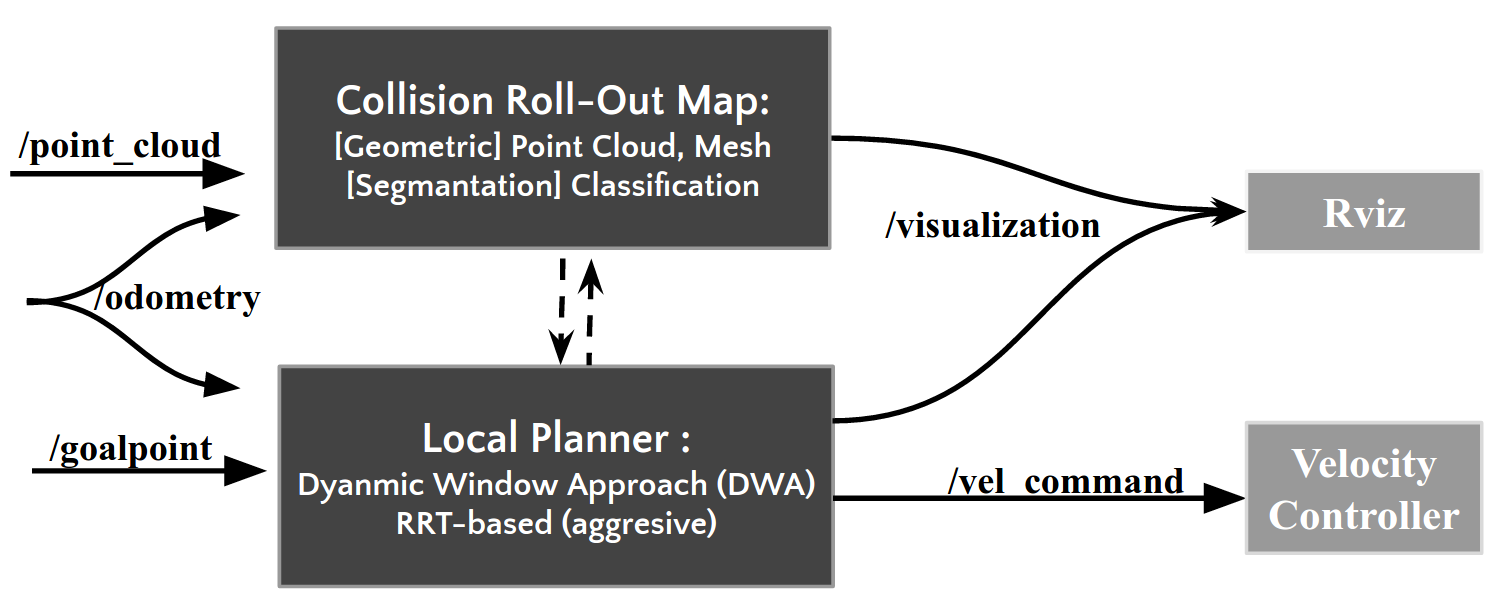
\includegraphics[width=0.8\columnwidth]{./RRTPlanner/fig/planner_module.png}}
		\caption{Block Diagram of our planner API.}
		\label{fig:planner_module}
	\end{center}
\end{figure} 

The block diagram of our planner modules is shown in Fig. \ref{fig:planner_module}, which can be separated into two modules with respect to functionality. The collision check module constructed a global simplified occupancy grid from vehicle current odometry and pure point cloud data, then communicated with RRT-based planner for collision check service. The velocity command is generated by planner and sent directly to the on-board velocity controller for execution. Visualization tools are also built via Rviz interface. The detail of two modules is described as follow:

\subsection{Collision Check Module}

Occupancy grid is a commonly-used data structure for obstacles detection. It stores one or multiple probabilities in each grid cell, and increases or decreases them based on sensor model. Since our testing scenario is relatively flat without noise, a simplified version of occupancy grid is used in the matter of fast implementation, in which we replaced the probabilities with a counter. Three different methods for obstacles segmentation were investigated and described below:

\begin{figure}[t]
	\centering
	\begin{subfigure}[b]{0.3\linewidth}
		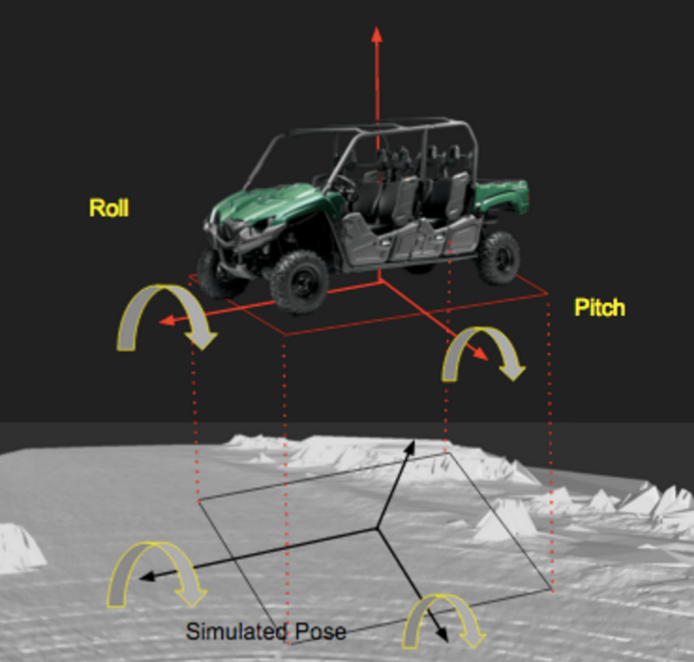
\includegraphics[width=\columnwidth]{./RRTPlanner/fig/mesh.png}
		\subcaption{Mesh with ODE simulation}
		\label{fig:collision_mesh}
	\end{subfigure}
	\begin{subfigure}[b]{0.3\linewidth}
		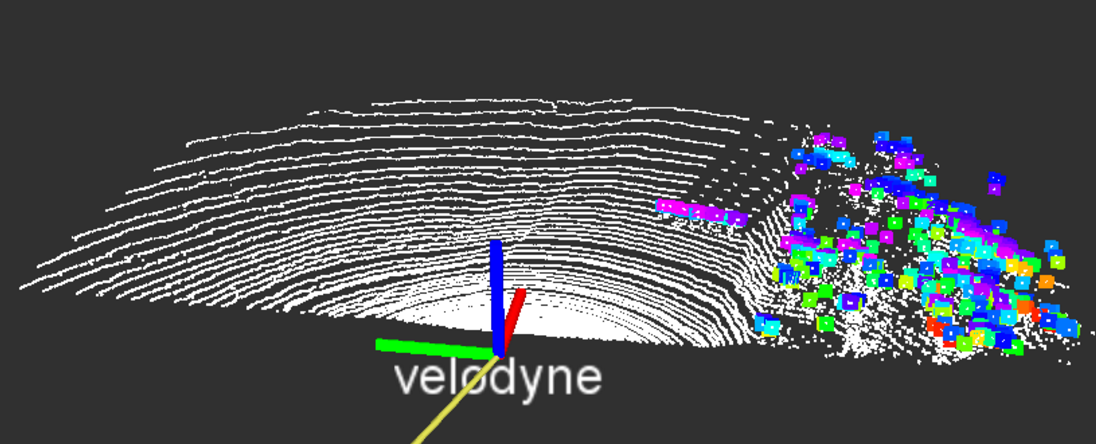
\includegraphics[width=\columnwidth]{./RRTPlanner/fig/ransac.png}
		\subcaption{RANSAC segmentation.}
		\label{fig:collision_ransac}
	\end{subfigure}
	\begin{subfigure}[b]{0.3\linewidth}
		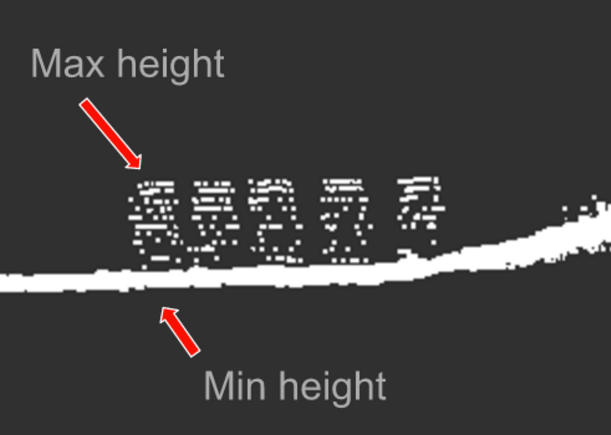
\includegraphics[width=\columnwidth]{./RRTPlanner/fig/height_map.png}
		\subcaption{Height map algorithm}
		\label{fig:collision_height_map}
	\end{subfigure}
	\caption{Three different methods of collision check. Note that for (b), the original and the the processed point cloud is represented with white and colored dot, respectively.}
    \label{fig:collision}
\end{figure}


\subsubsection{i. Mesh Representation with Simulation in Open Dynamic Engine (ODE)}
The original method implemented on the vehicle uses ODE and mesh data to simulate the vehicle pose on the ground. Collision is reported if an intersection was detected between vehicle and mesh or the simulated roll and pitch were beyond user-defined thresholds. 

\subsubsection{ii. Plane Removal with RANSAC Segmentation}
The second approach for collision check module is using RANSAC segmentation from Point Cloud Library (PCL) to fit the plane model. In our case, the plane model is the ground of our testing environment. We extract the outliers from RANSAC for obstacle detection. As shown in Fig. \ref{fig:collision_ransac}, the whtle point cloud is the original data from Velodyne Lidar. The colorful point cloud is the outliers from RANSAC. 

\subsubsection{iii. Height Map Algorithm}
The third method we used is height map algorithm. This is a simple and efficient algorithm in terms of computation. It calculates the height differences within one grid. If the height difference is greater than user-defined threshold, it will be categorized as an obstacle. As shown in Fig. \ref{fig:collision_height_map}, the artificial obstacle is approximately 1.5 meters. We set the threshold to be 1 meter. Thus it will be recognized as an obstacle. 

Since collision check is the most computationally expensive part of our system and we cannot afford to collide our platform with the obstacles. Efficiency and reliability are the most important requirements. The mesh representation is a good approach for future application such as driving on rough terrain. However, it was not feasible for our scenario in terms of computation consumption. The RANSAC segmentation is sensitive to off-road conditions; the plane model cannot be perfectly fit on rough terrain. In addition, the dusty environment in off-road driving create noises and interference to the Lidar. Considering our requirements and the discussion mentioned above, we choose height map algorithm as our final approach. It’s the fastest and the most reliable. Furthermore, to optimize the computing efficiency, we used bitwise operation instead of multiplication and the obstacle size are dilated to increase robustness of our system. 

\subsection{RRT-based Planner Module}

\begin{figure}[t]
	\begin{center}
		\centerline{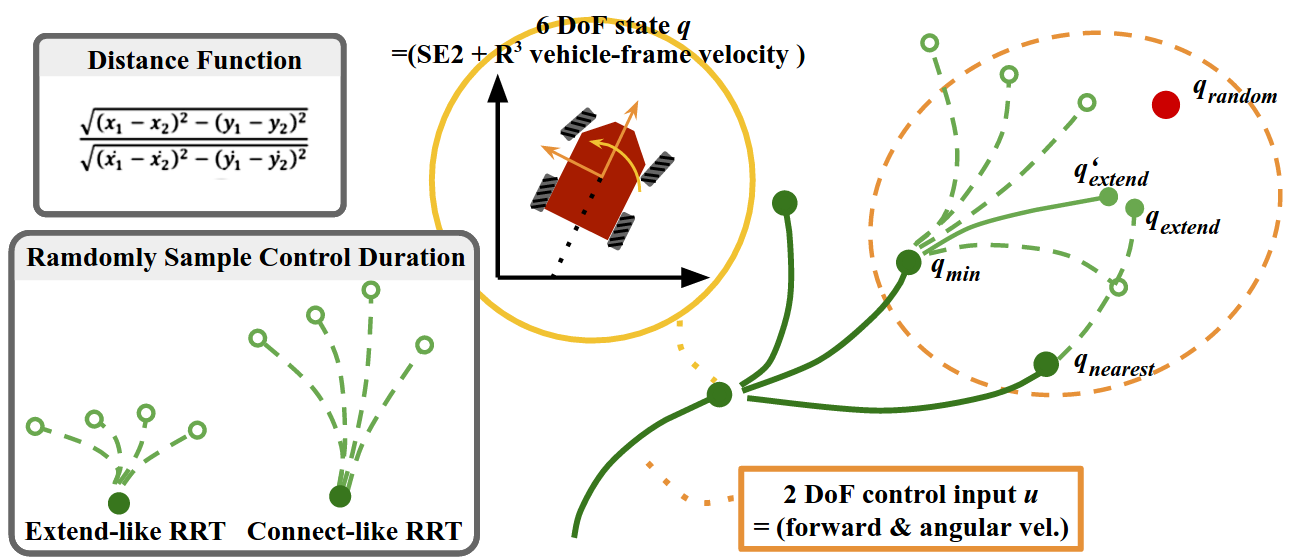
\includegraphics[width=0.8\columnwidth]{./RRTPlanner/fig/rrt.png}}
		\caption{The visualization of RRT-based planner.}
		\label{fig:rrt}
	\end{center}
\end{figure} 

\begin{figure}[t]
	\centering
	\begin{subfigure}[b]{0.7\linewidth}
		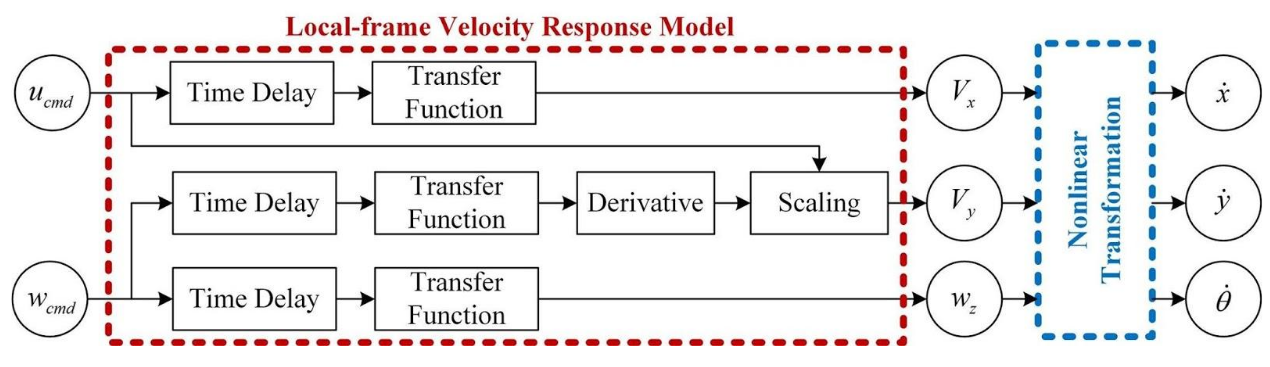
\includegraphics[width=\columnwidth]{./RRTPlanner/fig/vehicle_model_block.png}
		\subcaption{}
		\label{fig:vehicle_model_block}
	\end{subfigure}
	\begin{subfigure}[b]{0.28\linewidth}
		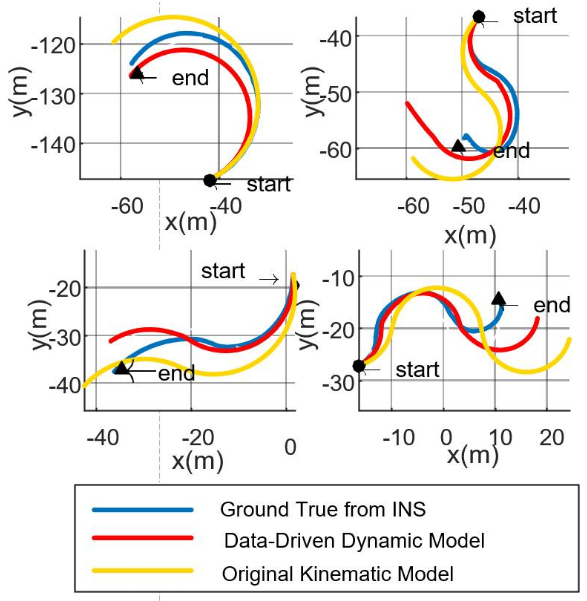
\includegraphics[width=\columnwidth]{./RRTPlanner/fig/vehicle_model_plot.png}
		\subcaption{}
		\label{fig:vehicle_model_plot}
	\end{subfigure}
	\caption{(a) Data flow of vehicle dynamic response model. The model takes two velocity control commands as input and estimates the velocity response in vehicle frame. (b) Comparison between data-driven dynamic model and original kinematic model. Note the time interval in each graph is 20 seconds.}
    \label{fig:vehicle_model}
\end{figure}


Instead of using traditional search-based planner such as A* or D*, we use a sample-based planner as our development platform. This critical choice comes from an insight that sample-based planner is more efficient for solving a high dimensional planning problem, which gives us a powerful tool when we want to utilize a more complex dynamic vehicle model for state propagation. Besides, maneuvering in wilderness can be seen as a generalized planning problem where discretizing the world based on resolution might not generate a smooth path.

% TODO cite OMPL
Simulation was first conducted within Open Motion Planning Library (OMPL) framework to investigate the performance among different sample-based planners. We used OMPL.app to simulate the behavior of different planners based our vehicle model and a specific map. Also, we used a benchmark tool provided by OMPL to compare the performance of different planners with different parameters. It turned out RRT planner is one of the competitive candidates. Since all of us are more familiar with RRT planner, we decided to use it as our baseline planner. 

Fig \ref{fig:rrt} visualizes the RRT tree. Each node represents a $6$ DoF states $q=[x,y, \theta ,v_{forward}, v_{sliding}, w]^T$, where the first three terms stand as a SE2 state space, and the last three terms stand as a vehicle-frame velocity in 2D plane. For control space, we utilize velocity control input, i.e. 2 DoF including forward and angular velocity, since it is commonly-used for autonomous ground vehicle, and is already built on the current vehicle controller system. 

In order to overcome the unpredictable characteristic of vehicle dynamic in off-road environment, an experimental-based model was addressed via field testing. More specifically, data is collected on field among different set of control inputs, then a predictive model $\dot{x}=f(x,u,t)$ is constructed off-line with standard system identification process. As shown in Fig. \ref{fig:vehicle_model_block}, the dynamic response of each velocity component at vehicle-frame is modeled as a first/second-order transfer function with time delay. Since the data-driven vehicle response model gives us a good estimation of the sliding velocity, which could plays a non-negligible role in off-road cases, it shows in Fig \ref{fig:vehicle_model_plot} a sufficient state estimation result when compared with the original kinematic model.

As a standard procedure of RRT in control space, a control input set and its operation duration should be determined in order to propagate toward an extended state after a random state is sampled. We first uniformly sampled the forward velocity command within an adjustable region. This command region is determined at each iteration based on previously issued command, current vehicle status, and previous executed path such that the vehicle will hold the velocity consistency without jerky output. Then, shooting method [X]\todo{} is used to determined the angular velocity command. Another modification we applied is the random sampling of control duration (see Fig. \ref{fig:rrt}). The initial thought came from our simulations in Section III\todo{fix this}, where we discovered choosing either extended-like RRT or connected-like RRT stands as an crucial factor for solving different maze scenarios. We believe loosening the constraint with such randomly sample mechanism will generalize our planner for various problems. % TODO section III

Finding an optimal plan is crucial for motion planning but computationally expensive if using a sample -based control-space planner. To overcome it, we implemented a time-optimal RRT* work from Frazzoli \cite{}. Moving from RRT toward RRT* includes two more optimization steps in each iteration: reconnecting of extended state, and tree edges trimming. For this project \todo{remove this}, only the first of two optimization steps was implemented because the trimming process in the second step includes updating the whole children tree, which will trade off with planning time. Since it is almost impossible to propagate to the same state in 6 DoF state space, the re-connection process from extended state to minimal-cost state instead of nearest state will require updating the extended state (i.e.  $q^{'}_{extend}$ $q_{extend}$ in Fig. \ref{fig:rrt}) if they are close enough. Last, since we would like to minimize our traveling time, the traveling time is estimated when calculated distance instead of Euclidean distance in 2D state space. 

The re-planning process is designed as follow: at the beginning of each planner loop, vehicle status, collision check map, and goal point are updated to formulate a RRT control-space planning problem. Then, we solved such problem many times and published the best one we had so far when the planner loop terminates. There is no tree maintenance process, i.e. we throw away the whole RRT tree, in each solving process. Though re-generating the whole RRT tree makes no sense at first glance, in practical we found out such design  can prevent the planner from publishing poor solution if bad tree structure was built at the beginning of growing stage. We admitted that if an optimal solution can be obtained from one single shot, the replanning setting would have changed significantly. Since there is a time delay between when vehicle status is updated and when the velocity command generated by RRT-based planner is executed, we utilize the same data-driven dynamic model to estimate the vehicle state after such time delay. The parameters used in our local planner are listed in TABLE I. 


\section{Experiments}

\subsection{Platform Introduction}

\begin{figure}[t]
	\begin{center}
		\centerline{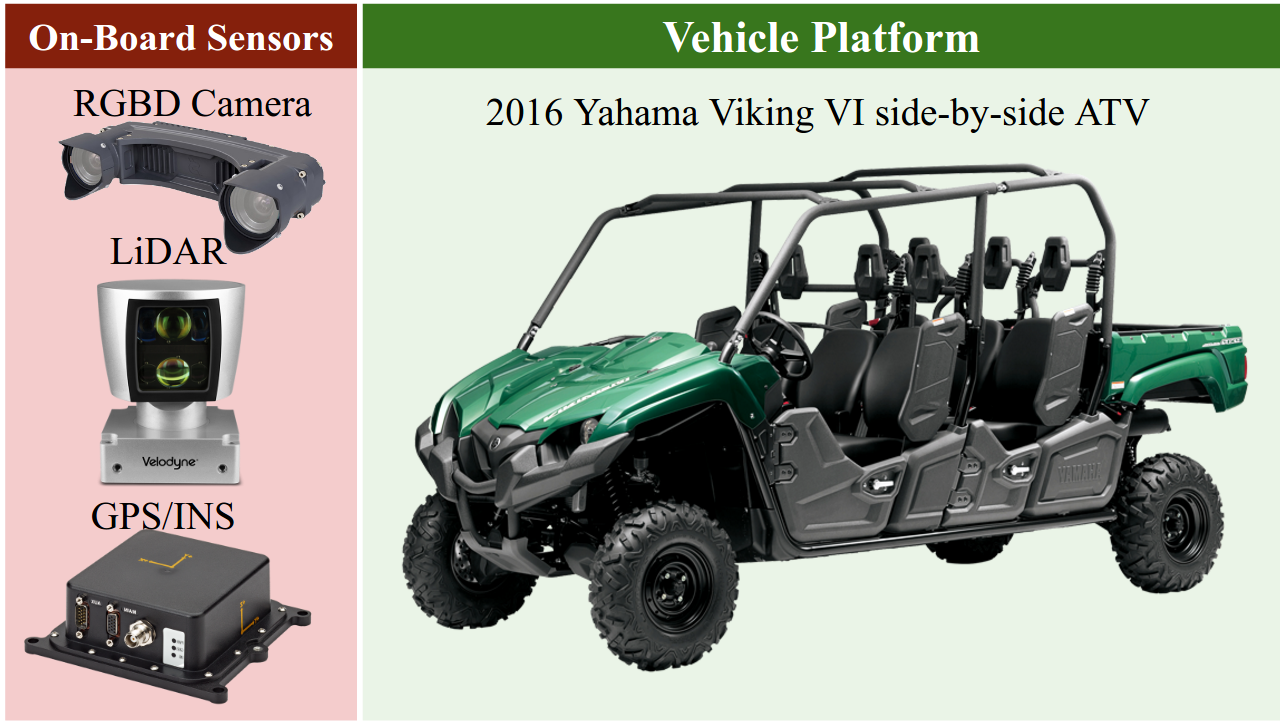
\includegraphics[width=0.8\columnwidth]{./RRTPlanner/fig/viking.png}}
		\caption{The testing vehicle platform and the on-board sensor.}
		\label{fig:viking}
	\end{center}
\end{figure} 

Our platform comes from an undergoing project at Robotics Institute cooperated between Field Robotics Center (FRC) and Yamaha Motor Company, which aimed to develop an autonomous vehicle for off-road driving in wilderness environment. Yamaha Viking VI side-by-side ATV is served as our main testing platform, which is shown in Fig. \ref{fig:viking}. The vehicle is equipped with custom drive-by-wire system, velocity controller, and navigation sensors such as GPS/INS, LiDAR, and RGB-D camera. Currently developing software modules include classification, pose estimation, global and local planner. 

Our testing scenario is designed as followed : the vehicle should perform S-shape maneuvering without collision with any static obstacles based on a model-based local planner. Standard operating speed ranges from $10$ to $40 kph$ ; the baseline testing speed in our case is set as $20 kph$ with the top speed of $30 kph$.


\subsection{Results}

\begin{figure}[t]
	\begin{center}
		\centerline{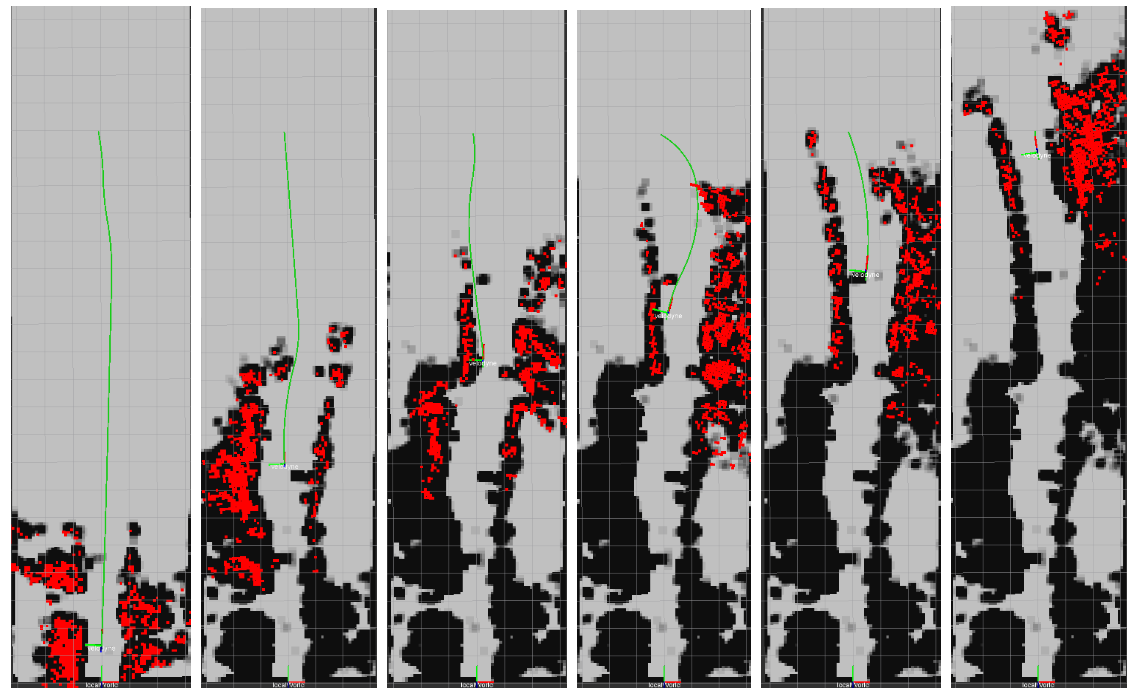
\includegraphics[width=0.8\columnwidth]{./RRTPlanner/fig/demo.png}}
		\caption{Screenshots of planner visualization output. The green path is the trajectory where each point is encoded with a 6 DoF state, 2 DoF control input, and a control duration. The red points are the filtered point cloud segmented as obstacles.}
		\label{fig:demo}
	\end{center}
\end{figure} 

Experiments were conducted on field to show the feasibility of our approach. Three 3-meter-length static obstacles were placed on the sides of a rectangle shaped field with 10-meter width and 150-meter length. The vehicle successfully avoided all the obstacles at 20 kph. However, driving at higher speed (~30kph) sometimes made collision map vulnerable to noise such as dust and sand blow up when the vehicle drove through, which highly affect the path quality outputted by planner. The example of planning path generation is visualized in Fig. . We have recorded some videos on-line: \footnote{Simulation in OMPL.app: \url{http://ppt.cc/sBLAh
}} \footnote{On-field testing with path visualization: \url{https://youtu.be/LibnO8_Sjm0}}

\subsection{Conclusion}

A RRT-based local planner for high-speed maneuvering is proposed for the application off-road navigation. Several methods are investigated for obstacle detection, with the final version implemented with height map algorithm. A simplified version of occupancy grid is built in global frame when vehicle is moving. Several modifications is implemented in order to obtain the minimal traveling-time trajectory, with a data-driven vehicle model is utilized for state propagation. Our planner can successfully avoid three obstacles on turnpike with vehicle velocity up to 30 kph. Future works include constructing a more complex model in 3D space, strengthening the collision map with more informative data such as mesh, or classification segmentation, and planner optimization. 



\end{document}